% This is "bach-ref-2009.tex" Updated january 29th 2010.
% This file should be compiled with "sig-alternate-fixed.cls" January 2010.
% It is based on the ACM style "sig-alternate.cls"
% -------------------------------------------------------------------------
% This example file demonstrates the use of the 'sig-alternate-fixed.cls'
% V2.5 LaTeX2e document class file. It is for those submitting
% articles to the Twente Student Conference on IT. Both this file as the 
% document class file are based upon ACM documents.
%
% ----------------------------------------------------------------------------------------------------------------
% This .tex file (and associated .cls) produces:
%       1) The Permission Statement
%       2) The Conference (location) Info information
%       3) The Copyright Line TSConIT
%       4) NO headers and/or footers
%
%
% Using 'sig-alternate.cls' you have control, however, from within
% the source .tex file, over both the CopyrightYear
% (defaulted to 200X) and the ACM Copyright Data
% (defaulted to X-XXXXX-XX-X/XX/XX).
% e.g.
% \CopyrightYear{2007} will cause 2007 to appear in the copyright line.
% \crdata{0-12345-67-8/90/12} will cause 0-12345-67-8/90/12 to appear in the copyright line.
%
% ---------------------------------------------------------------------------------------------------------------
% This .tex source is an example which *does* use
% the .bib file (from which the .bbl file % is produced).
% REMEMBER HOWEVER: After having produced the .bbl file,
% and prior to final submission, you *NEED* to 'insert'
% your .bbl file into your source .tex file so as to provide
% ONE 'self-contained' source file.
%

% refers to the cls file being used
\documentclass{sig-alternate-br}

%USING SIGCOM TEMPLATE
%\documentclass[sigconf,natbib=true]{acmart}
%\settopmatter{printacmref=false} % Removes citation information below abstract
%\renewcommand\footnotetextcopyrightpermission[1]{} % removes footnote with conference information in first column
%\pagestyle{plain} % removes running headers
%-------------------------------------------------------------------------------
% PACKAGES 
%-------------------------------------------------------------------------------
%\usepackage{comment}
\usepackage{xcolor}
\usepackage{natbib}

%-------------------------------------------------------------------------------
% PACKAGES FOR URL
%-------------------------------------------------------------------------------
\usepackage{hyperref}
\hypersetup{colorlinks, citecolor=blue, filecolor=blue, linkcolor=blue, urlcolor=blue}
\usepackage{breakurl}
%\usepackage[hyphens]{url}

%-------------------------------------------------------------------------------
% PACKAGES AND COMMANDS FOR TABLES 
%-------------------------------------------------------------------------------
\usepackage{tabularx}
\usepackage{longtable}
\usepackage{multirow}
\usepackage{adjustbox}
\usepackage{color,colortbl,xcolor}
\usepackage{array}
\newcolumntype{L}[1]{>{\raggedright\let\newline\\\arraybackslash\hspace{0pt}}m{#1}}
\newcolumntype{C}[1]{>{\centering\let\newline\\\arraybackslash\hspace{0pt}}m{#1}}
\newcolumntype{R}[1]{>{\raggedleft\let\newline\\\arraybackslash\hspace{0pt}}m{#1}}
%-------------------------------------------------------------------------------
% PACKAGES FOR FIGURES
%-------------------------------------------------------------------------------
\usepackage{graphicx,graphics,float,subfigure,wrapfig,epstopdf}
\usepackage{dblfloatfix}%to fix the problem of [h!] [t!] [!b]
\epstopdfsetup{update}
%-------------------------------------------------------------------------------
% PACKAGES FOR REFERENCE LIST FORMAT 
%-------------------------------------------------------------------------------
%\usepackage[square,numbers]{natbib}
%options: round; square; curly; angle; colon; comma; authoryear; numbers; 
%         super; sort; sort&compress; longnamesfirst; sectionbib; nonamebreak;

\def\BibTeX{{\rm B\kern-.05em{\sc i\kern-.025em b}\kern-.08emT\kern-.1667em\lower.7ex\hbox{E}\kern-.125emX}} 
% defining the \BibTeX command - from Oren Patashnik's original BibTeX documentation.

%-------------------------------------------------------------------------------
% PACKAGE FOR CREATING GANTT VISUALIZATION (PLANNING TABLE) 
%-------------------------------------------------------------------------------
\usepackage{soul}
\usepackage{libs/gantt} %for the planning table
%-------------------------------------------------------------------------------
% CREATING COMMANDS FOR AUTOREF 
%-------------------------------------------------------------------------------
\renewcommand{\chapterautorefname }{\S}
\renewcommand{\sectionautorefname}{\S}
\renewcommand{\subsectionautorefname}{\S}
\renewcommand{\subsubsectionautorefname}{\S}
\newcommand{\subfigureautorefname}{\figureautorefname}
%-------------------------------------------------------------------------------
% CREATING COMMANDS FOR MAKING COMMENTS
%-------------------------------------------------------------------------------
\newcommand\comment[1]{{\color{blue} \noindent\sffamily\textbf{[COMMENT: #1]}}}
%\renewcommand\comment[1]{{ \sffamily [xxx:  #1]}}
%-------------------------------------------------------------------------------
%-------------------------------------------------------------------------------

\begin{document}
%
% --- Author Metadata here --- DO NOT REMOVE OR CHANGE 
\conferenceinfo{28$^{th}$ Twente Student Conference on IT}{Febr. 2$^{nd}$, 2018, Enschede, The Netherlands.}
\CopyrightYear{2018} % Allows default copyright year (200X) to be over-ridden - IF NEED BE.
%\crdata{0-12345-67-8/90/01}  % Allows default copyright data (0-89791-88-6/97/05) to be over-ridden - IF NEED BE.
% --- End of Author Metadata ---

\title{PaperCake Recipe for Students}
% In Bachelor Referaat at University of Twente the use of a subtitle is discouraged.
% \subtitle{[Instructions]}

%
% You need the command \numberofauthors to handle the 'placement
% and alignment' of the authors beneath the title.
%
% For aesthetic reasons, we recommend 'three authors at a time'
% i.e. three 'name/affiliation blocks' be placed beneath the title.
%
% NOTE: You are NOT restricted in how many 'rows' of
% "name/affiliations" may appear. We just ask that you restrict
% the number of 'columns' to three.
%
% Because of the available 'opening page real-estate'
% we ask you to refrain from putting more than six authors
% (two rows with three columns) beneath the article title.
% More than six makes the first-page appear very cluttered indeed.
%
% Use the \alignauthor commands to handle the names
% and affiliations for an 'aesthetic maximum' of six authors.
% Add names, affiliations, addresses for
% the seventh etc. author(s) as the argument for the
% \additionalauthors command.
% These 'additional authors' will be output/set for you
% without further effort on your part as the last section in
% the body of your article BEFORE References or any Appendices.

\numberofauthors{2} %  in this sample file, there are a *total*
% of EIGHT authors. SIX appear on the 'first-page' (for formatting
% reasons) and the remaining two appear in the \additionalauthors section.
%
\author{
% You can go ahead and credit any number of authors here,
% e.g. one 'row of three' or two rows (consisting of one row of three
% and a second row of one, two or three).
%
% The command \alignauthor (no curly braces needed) should
% precede each author name, affiliation/snail-mail address and
% e-mail address. Additionally, tag each line of
% affiliation/address with \affaddr, and tag the
% e-mail address with \email.
%
% 1st. author
\alignauthor
Student name\\
       \affaddr{University of Twente}\\
       \affaddr{P.O. Box 217, 7500AE Enschede}\\
       \affaddr{The Netherlands}\\
	   \email{student@student.utwente.nl}
%\alignauthor
% Leandro M. Bertholdo\\
% 	   \affaddr{University of Twente}\\
%        \affaddr{P.O. Box 217, 7500AE Enschede}\\
%        \affaddr{The Netherlands}\\
% 	   \email{l.m.bertholdo@utwente.nl}\\
}
% There's nothing stopping you putting the seventh, eighth, etc.
% author on the opening page (as the 'third row') but we ask,
% for aesthetic reasons that you place these 'additional authors'
% in the \additional authors block, viz.
% \additionalauthors{Additional authors: John Smith (The
% Th{\o}rv{\"a}ld Group, email: {\texttt{jsmith@affiliation.org}})
% and Julius P.~Kumquat (The Kumquat Consortium, email:
% {\texttt{jpkumquat@consortium.net}}).}
% \date{30 July 1999}
% Just remember to make sure that the TOTAL number of authors
% is the number that will appear on the first page PLUS the
% number that will appear in the \additionalauthors section.

\maketitle
%-------------------------------------------------------------------------------%
\begin{abstract}
The structure of an abstract should have the (i) context, (ii) problem, (iii) how your proposal is different from the literature (without saying what you propose), (iv) your proposal, and (v) your most astonishing finding (or [if proposal] your expected scientific contribution(s)). Your goal is to meet $\pm$100 words. The ``context'' part describes what your reader should know to understand your research. The ``problem'' part describes why your research need to be done; why it is interesting; and why someone needs to spend time reading your work. In the ``how your proposal is different'' you should say what is the main issue in similar works that you intend to solve. The ``proposal'' part describes what your proposal and the overall methodology to achieve your proposal (goal). Finally, your ``findings'' part I recommend you to surprise your reader, make him VERY interested to read your paper. If your ``findings'' part is related to a proposal document then you should describe what do you expect (intend) to be your scientific contribution.
\end{abstract}

\keywords{Keywords are your own designated keywords.}

\section{Introduction} 
\label{sec:introduction}

\comment{The Introduction section has more or less the same structure as your abstract. The difference is that in the abstract each part is one statement/phrase, while in the introduction each part is a paragraph. So, (i) context, (ii) problem, (iii) proposal, and your most astonishing (iv) finding. Of course in the Introduction section you can give far more details than in the abstract. Avoid to copy and paste statements, re-write with different words.}

\comment{In addition to the structure that you already know you should include your \textit{research questions} between the ``proposal'' paragraph and the ``findings''. The statement that precede the RQ is something like the following: }

To pursue our goal, we have defined the following research questions (RQ) as the basis of our research: 
\begin{itemize}	
	\item \textbf{RQ1:} What are ..?
	\item \textbf{RQ2:} How to ... ?
	 \item \textbf{RQ3:} How to ...?
\end{itemize}



\comment{Please, avoid "yes or no" questions. Make questions that your reader are not able to answer immediately. Usually the questions depend on each other, it means that to answer one question you must answer the one before.}

\comment{Before a little bit of your most astonishing findings you must to introduce the structure of your paper (or proposal). Usually the text looks like the following.}
 
``The remainder of this paper (or proposal) is organized as follows. Section 2 will discuss the approaches expected for answering each research question. After that, we present a preliminary planning for the research questions in Section 3. Finally, we conclude with a proposal and planning for the thesis structure in Section 4.'' 






\section{Related Work}

\begin{enumerate}
\item Go to Google scholar and search using \textbf{set of keywords} related to your research. How many entries resulted from those sets? put this in a excel sheet.
\item (For each set of keywords) copy and paste the top 20 titles of papers (from Google Scholar) in a Excel. Judge whether the title has something similar to the work that you intend to do. Update the excel file.
\item From the similar/interesting papers (based-on-title), read their abstracts. In the Excel file mark which papers have interesting abstracts. 
\item Each paper with interesting titles and abstracts, you should read the introduction and mark on Excel which have an interesting introduction.
\item Papers with interesting titles, abstracts, and introduction, you should read the conclusion and mark on Excel which have an interesting conclusion.
\item The papers that are interesting till this point you should read the entire paper! Update the Excel what are the similarities with the other papers and what are the differences.
\item Create a table and place it in the 'Related Work' section of your proposal/paper/thesis. This table should contain the reference to the paper, the similarities and the differences. 
\end{enumerate}

For the phase after the proposal you should re-read those interesting papers and take note of their "related work" papers. Read those papers and update the Excel Sheet.

\textbf{NOTE: that the final goal of this section is a table that summarizes the characteristics of each paper and your critical analysis to highlight the existing gaps of research.}

Examples of how to make a reference:
\begin{itemize}
	\item $\backslash$citep outputs: \citep{jjsantanna2015IM1}
	\item $\backslash$citet outputs: \citet{jjsantanna2015IM1}

\end{itemize}

\section{Methodologies}
<brief summary explaining the content and the connection><you could even to make a picture explaining how the parts connect for example a conceptual figure with your idea (if possible). On this, I must say that Figures MUST be in pdf format (I like to use Inkscape to create my figures, then I export to pdf) [ask me how, for help]> 

\subsection{On answering RQ1}

\subsection{On answering RQ2}

\subsection{On answering RQ3}
\begin{figure}[h!]
	\label{fig:approach}
	\centering
	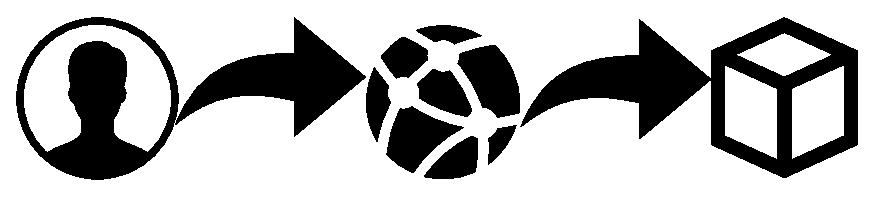
\includegraphics[width=0.45\textwidth]{figs/example.eps}
	\caption{Example of Figure.}
\end{figure}

\section{Planning}
 In this section we will shortly discuss the planning of the study. The study has been split into six parts, as can be seen in the table below. Note that a planning such as this when is to be seen as a guideline. There are however some hard deadlines for handing in drafts and final versions. Here we have an overview of the deadlines:
 \begin{itemize}	
	\item December 1st: Final proposal submission
	\item January 19th: Draft paper submission
	\item January 26th: Final paper submission
	\item January 31th: Conference presentation
\end{itemize}
The planning is made in order to adhere to these submission deadlines.

% More examples on how to do a planning table you can see in \url{http://www.martin-kumm.de/wiki/doku.php?id=05Misc:A_LaTeX_package_for_gantt_plots}

\begin{figure}[ht]
\noindent\resizebox{0.49\textwidth}{!}{
\begin{gantt}[xunitlength=0.5cm,fontsize=\small,titlefontsize=\small,drawledgerline=true]{15}{12} %(1)lines (2)columns
		
		\begin{ganttitle} %Month
			\titleelement{\textbf{Planning Table}}{12}
		\end{ganttitle}
		
		\begin{ganttitle} %Month
			\titleelement{November}{3}
			\titleelement{December}{5}
			\titleelement{January}{4}
		\end{ganttitle}
		\begin{ganttitle} % Week number
			\numtitle{1}{1}{12}{1}
		\end{ganttitle}
		\ganttbar[color=gray]{Proposal}{0}{3}
		\ganttmilestone[color=orange]{Draft proposal}{2}
		\ganttmilestone[color=red]{Final proposal}{3}
		\ganttbar[pattern=grid,color=orange]{Writing}{3}{8}
		\ganttbar[color=blue]{RQ1}{3}{1}
		\ganttcon{3}{3}{3}{7}
		\ganttbarcon[color=blue]{RQ2}{4}{2}
		\ganttbar[pattern=grid,color=red]{Holidays}{6}{2}
		\ganttbar[color=blue]{RQ3}{8}{2}
		\ganttcon{6}{8}{8}{10}
		\ganttbarcon[color=blue]{RQ4}{10}{1}
		\ganttmilestone[color=orange]{Draft Paper submission}{10}
		\ganttmilestone[color=red]{Final Paper submission}{11}
		\ganttbar[color=green]{Presentation}{11}{1}
		\ganttcon{11}{11}{11}{14}

\end{gantt}	
} 
\end{figure}



% The research topics part consists solely of a literature study that focuses on ... All relevant information learned from this will be integrated in a survey that will form the first part of the thesis.

% Following the research topics are each of the research questions, with time allotted at the end of each research question to integrate the results into the thesis. 

\section{Results}

\section{Conclusions}

%-------------------------------------------------------------------------------%
%-------------------------------------------------------------------------------
%\newcommand{\newblock}{}

\def\UrlBreaks{\do\/\do-}
\bibliographystyle{abbrvnat} %abbrvnat OR unsrtnat OR plainnat
\bibliography{my_bibliography}
%-------------------------------------------------------------------------------%
%-------------------------------------------------------------------------------
\newpage\newpage
\section*{IMPORTANT NOTES and TIPS:}

\begin{itemize}
	\item I DO recommend: "PhD: How to write a great research paper." % \url{https://www.youtube.com/watch?v=1AYxMbYZQ1Y} (updated on 17/01/2019)
	\item Figures MUST be in svg, eps, or pdf format (I like to use Inkscape to % create my figures, then I export to pdf);
	\item Graphs could be plotted using gnuplot but I prefer anything from jupyter % notebook; 
	\item Avoid vague words: relatively, possible, ... 
	\item Be quantitative! give an idea of numbers.
	\item Avoid start with 'because'
%	\item To reference something you can do like this: \citep{justyna2015SBRC}, % \citep{kerkers2014aims}, or \citet{jjsantanna2015IM2,jjsantanna2015IM1}, \citet{santanna2013aims} \comment{Look how I did in the latex file}

\end{itemize}

\balancecolumns
\end{document}

